\documentclass[
aspectratio=169 % comment for 4:3
]{beamer}

\newcommand{\cmd}[1]{\texttt{\textbf{#1}}}
\newcommand{\args}[1]{\texttt{\textit{#1}}}

\usetheme[
hidetotal, % hide the total number of slides on the bottom right
hidenumbers, % hide current slide number
% hidename, % hide author name and title in footline
hidebullets, % use empty bullets in itemize
hidefootline, % hide the footline
%
% the previous options allow for a minimalistic style as recommended by Patrick
% Winston in his "how to speak" lecture at MIT
%
% sidebar, % show sidebar
hugetitle, % print main title in huge font
% thin, % use a thinner font
% bold, % use bold titles
% standardtitle, % use standard title slide (no picture)
]{mfrancois}

\setsecondarylogo{title/isia-logo} % Add a secondary logo to the title slide, optional
\settitleimage{title/raspberry} % Change the title slide image, optional (use images with a ratio identical to the one provided)

\author[F. Marelli]{François Marelli}
\affiliation[UMONS]{UMONS, ISIA Lab}
\title{Atelier Créactifs: Raspberry Pi}
\subtitle{Séance 3: Python et l'interface GPIO}
\extras{
\includegraphics[height=25pt]{title/creactifs}}
\date{2 mars 2026}

\graphicspath{{images}}

\begin{document}

\maketitle

\begin{frame}{L'interface GPIO}{General Purpose Input/Output}
    \centering
    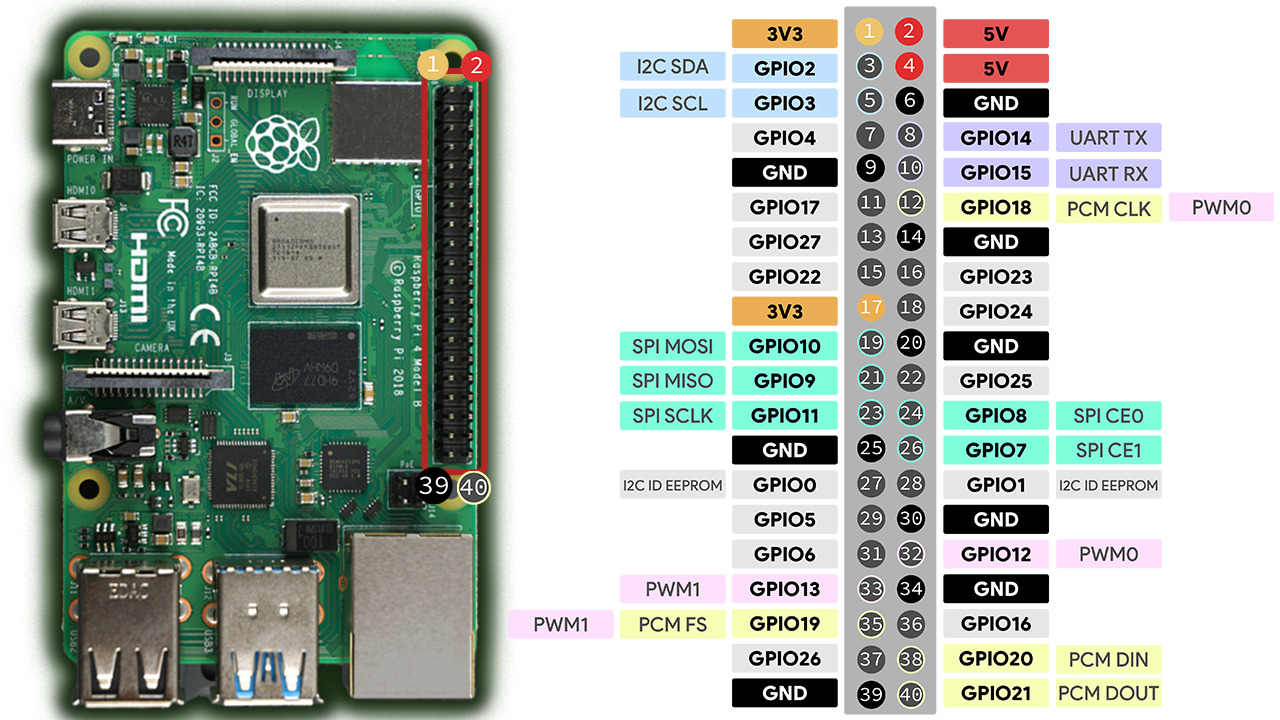
\includegraphics[width=.75\textwidth]{pinout}

    \tiny{Source: randomnerdtutorials.com}
\end{frame}

\begin{frame}{Un circuit simple}{Une entrée et une sortie digitales}
    \begin{columns}
        \begin{column}{.6\textwidth}
            \centering
            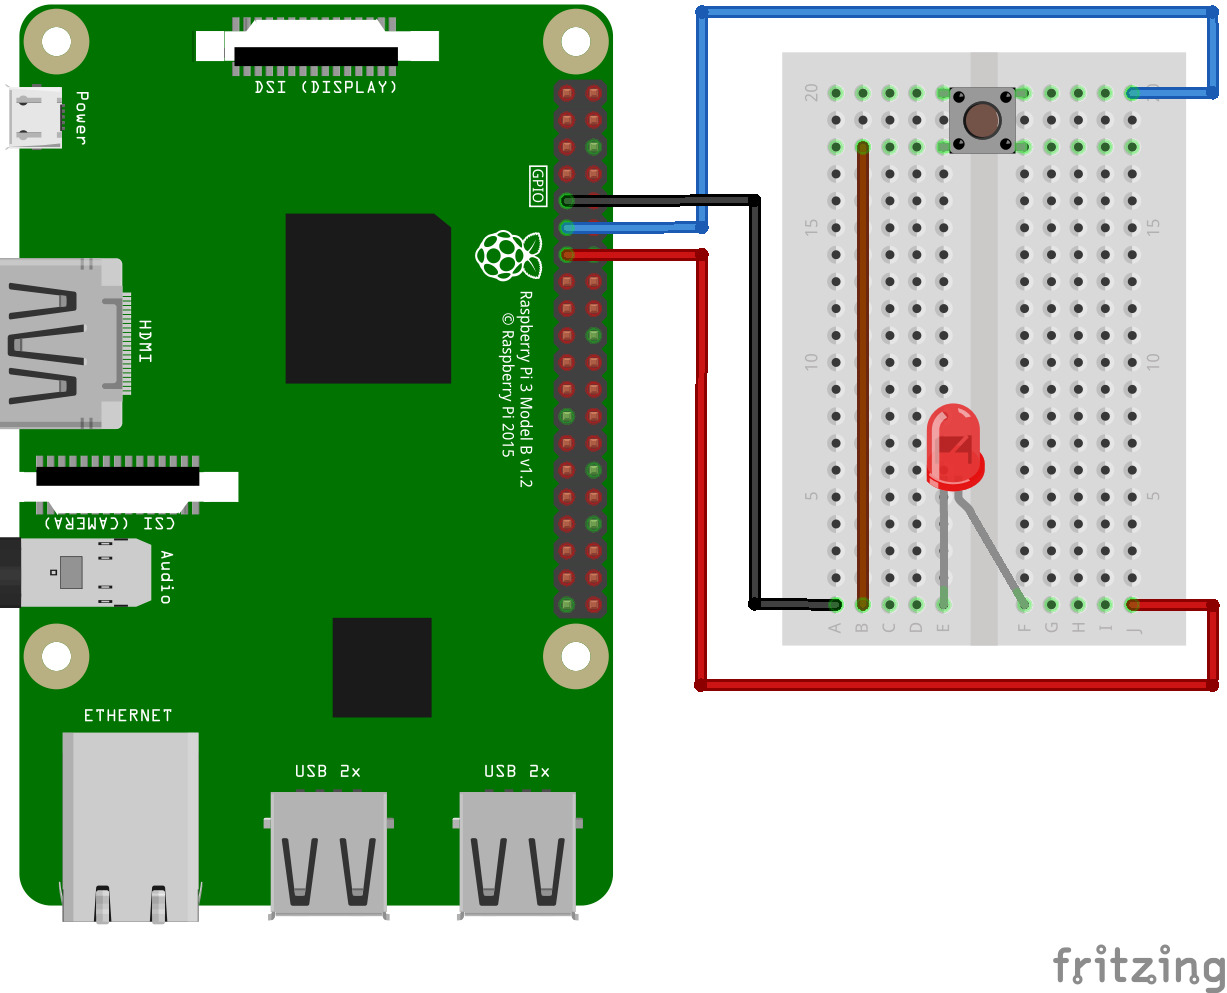
\includegraphics[width=.9\textwidth]{breadboard}
        \end{column}
        \begin{column}{.4\textwidth}
            Contact par ligne de 5
            \bigskip

            Attention au sens de la LED!
        \end{column}
    \end{columns}
\end{frame}

\begin{frame}{Un circuit simple}{Une entrée et une sortie digitales}
    \begin{columns}
        \begin{column}{.45\textwidth}
            \centering
            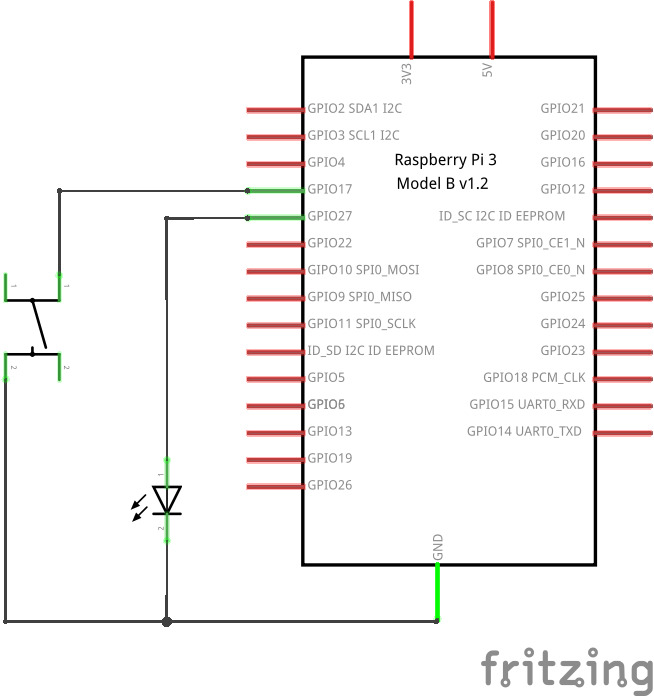
\includegraphics[width=.9\textwidth]{schematic}
        \end{column}
        \begin{column}{.5\textwidth}
            Schéma du circuit précédent
            \bigskip

            Le bouton (à gauche):
            \begin{itemize}
                \item par défaut: pas de contact
                \item pressé: contact entre GPIO17 et GND
            \end{itemize}

            \bigskip
            La LED (à droite):
            \begin{itemize}
                \item allumée si GPIO27 est à 3.3V
                \item éteinte si GPIO27 est à 0V
            \end{itemize}

        \end{column}
    \end{columns}
\end{frame}

\begin{frame}{Python}{Un langage de programmation}
    \begin{columns}
        \begin{column}{.35\textwidth}
            \centering
            
\includegraphics[width=.9\textwidth]{python}
        \end{column}
        \begin{column}{.6\textwidth}
            Haut niveau
            \begin{itemize}
                \item plus simple à aborder
                \item prototypage rapide
            \end{itemize}

            \medskip
            Interprété
            \begin{itemize}
                \item pas de compilation
                \item multiplateforme
            \end{itemize}

            \medskip
            À usage général
            \begin{itemize}
                \item très flexible
                \item large écosystème de librairies
            \end{itemize}
        \end{column}
    \end{columns}
\end{frame}

\begin{frame}[fragile]{Premier programme Python}{Bases de programmation}
    \cmd{nano}\args{ hello.py}: créer un premier code Python

    \bigskip

    \begin{lstlisting}
print("Hello, world!")
    \end{lstlisting}
    \medskip

    \cmd{python}\args{ hello.py}: exécuter le code

    \bigskip
    Sur Raspberry Pi OS, on peut utiliser \textit{Geany} pour écrire du code

    \bigskip
    \alert{Attention! Les indentations (espaces \textbf{OU} tabs) sont cruciales
        en Python!}

\end{frame}

\begin{frame}[fragile]{Retenir l'information: les variables}
    \begin{lstlisting}
# Ceci est un commentaire, il est ignore par Python
# Les variables permettent de stocker de l'information

# Par exemple, un nombre
nombre = 42.0

# Ou du texte, entre " ou '
texte = "Voici du texte"

# Ou une valeur logique
vrai = True
faux = False

# On peut effectuer des operations et modifier les variables
nombre = (nombre - 5) * 3 / 2 + 1
\end{lstlisting}
\end{frame}

\begin{frame}[fragile]{Regrouper des variables: les listes et dictionnaires}
    \begin{lstlisting}
# Une liste peut contenir plusieurs variables differentes
liste = [42, "texte", True]

# On utilise [] pour acceder a un element, en partant de 0
print("liste[1] =", liste[1])

# On peut ajouter des elements a la fin de la liste
liste.append(3.14)
print("liste apres append:", liste)

# Et mesurer sa longueur
longueur = len(liste)
print("longueur de la liste:", longueur)

# Un dictionnaire associe chaque element a une cle
dictionnaire = {"univers": 42, "pi": 3.14}
print("dictionnaire['univers'] =", dictionnaire["univers"])
\end{lstlisting}
\end{frame}

\begin{frame}[fragile]{Faire des choix: les conditions}
    \begin{lstlisting}
compteur = 0 

# Les conditions permettent de faire des choix dans le programme
if compteur > 5:
    print("Compteur est strictement plus grand que 5")

# elif est une seconde condition, si la premiere est fausse
elif compteur == 5:
    print("Compteur vaut 5")

# on peut combiner les operateurs logiques and, or, not
elif (False or True) and not True:
    print("Ceci ne se produira pas")

#else est la condition par defaut, si le autres sont fausses
else:
    print("Compteur <= 5")
\end{lstlisting}
\end{frame}

\begin{frame}[fragile]{Répéter des opérations: les boucles}
    \begin{lstlisting}
compteur = 0

# Les boucles while tournent tant que la condition est vraie
while compteur < 10:
    print("Compteur:", compteur)
    compteur = compteur + 1  

# Les boucles for iterent sur une sequence d'elements
for index in range(5):
    print("index:", index)

# On peut "casser" une boucle en avance avec break
while True:
    print("Ceci tourne pour toujours")
    compteur = compteur + 1

    if compteur > 20:
        break
\end{lstlisting}
\end{frame}

\begin{frame}[fragile]{Réutiliser du code: les fonctions et librairies}
    \begin{lstlisting}
# Les fonctions peuvent etre appelees avec des arguments
# syntaxe: def nom_fonction(arguments):
def ajouter(a, b):
    print("Addition de", a, "et", b)

    # Et retourner une valeur
    return a + b

resultat = ajouter(3, 4)
print("Resultat:", resultat)

# On peut importer des librairies pour utiliser des fonctions existantes
import math
resultat = math.sqrt(2)
print("Racine carre de 2:", resultat)
\end{lstlisting}
\end{frame}

\begin{frame}{\texttt{gpiozero}}{Une librairie simple pour contrôler les GPIO}
    \texttt{gpiozero} permet de contrôler les GPIO en Python facilement:
    \begin{itemize}
        \item Pré-installé sur Raspberry Pi OS
        \item API simple et intuitive
        \item Documentation complète et claire
              (\url{https://gpiozero.readthedocs.io/})
        \item Nombreux périphériques inclus (LED, bouton, moteurs, capteurs,
              etc.)
    \end{itemize}

    \bigskip
    Objectifs du jour:
    \begin{enumerate}
        \item Contrôler une LED
        \item Utiliser un bouton
    \end{enumerate}
\end{frame}

\begin{frame}[fragile]{Contrôler une LED}{Allumer et éteindre}
    \begin{lstlisting}
# On n'importe que ce dont on a besoin ici
from gpiozero import LED
from time import sleep

# Creer un objet LED sur le port GPIO27 (pin 13)
led = LED(27)

# Faire clignoter la LED 10 fois
for i in range(10):
    led.on()  # Allumer la LED
    sleep(0.5)  # Attendre 0.5 secondes
    led.off()  # Eteindre la LED
    sleep(0.5)
\end{lstlisting}
\end{frame}

\frame{\centering\huge{\alert{Comment varier la luminosité d'une LED controlée
            par une
            sortie digitale?}}}

\begin{frame}{Tricher avec le PWM}{Pulse Width Modulation}
    \begin{columns}
        \begin{column}{.6\textwidth}
            \centering
            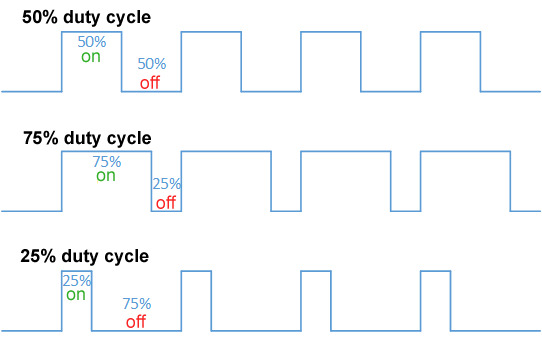
\includegraphics[width=.95\textwidth]{pwm}

            \tiny{Source: commons.wikimedia.org}
        \end{column}
        \begin{column}{.4\textwidth}
            Alternance haute vitesse 1/0

            \bigskip
            Trop rapide pour nos yeux

            \(\rightarrow\) impression d'analogique

            \bigskip
            Varier la largeur pour "l'intensité"
        \end{column}
    \end{columns}
\end{frame}

\begin{frame}[fragile]{Contrôler une LED}{Varier la luminosité avec le PWM}
    \begin{lstlisting}
from gpiozero import PWMLED
from time import sleep

# Creer un objet PWMLED sur le port GPIO27 (pin 13)
led = PWMLED(27)

# Faire clignoter la LED 10 fois
for i in range(10):
    led.value = 0.7 # Allumer la LED a 70% de luminosite
    sleep(0.5)  # Attendre 0.5 secondes
    led.value = 0.2 # Diminuer la luminosite a 20%
    sleep(0.5)

led.value = 0.0 # Eteindre la LED
\end{lstlisting}

    \smallskip
    Soyez créatifs, imaginez des motifs de clignotement (rampe, sinus, ...)!

\end{frame}

\begin{frame}[fragile]{Utiliser un bouton}{Lire la valeur manuellement}
    \begin{lstlisting}
from gpiozero import Button
from time import sleep

# Creer un objet Button sur le port GPIO17 (pin 11)
button = Button(17)

# Lire la valeur du bouton chaque seconde
for i in range(10):
    if button.is_pressed:
        print("Le bouton est appuye!")
    else:
        print("Le bouton n'est pas appuye.")
    sleep(1)
\end{lstlisting}
\end{frame}

\begin{frame}[fragile]{Utiliser un bouton}{Interrompre le programme quand on
        appuie}
    \begin{lstlisting}
from gpiozero import Button
from time import sleep

# Creer un objet Button sur le port GPIO17 (pin 11)
button = Button(17)

# Creer une fonction a executer quand on appuie sur le bouton
def on_press():
    print("Bouton appuye!")

# Associer la fonction a l'evenement "when_pressed" du bouton
button.when_pressed = on_press

input("Appuyez sur Enter pour terminer le programme...")
\end{lstlisting}
\end{frame}

\begin{frame}{Exercice de synthèse}{Contrôler la LED avec le bouton}
    Combiner les éléments \texttt{LED}/\texttt{PWMLED} et \texttt{Button}

    \bigskip
    Objectifs:
    \begin{enumerate}
        \item allumer la LED quand le bouton est appuyé
        \item éteindre la LED quand le bouton est appuyé à nouveau
        \item répéter
    \end{enumerate}

    \bigskip
    Bonus:
    \begin{itemize}
        \item utiliser le PWM pour allumer et éteindre la LED progressivement
        \item faire clignoter la LED tant que le bouton est appuyé
    \end{itemize}
\end{frame}

\begin{frame}{Le capteur DHT22}{Une mini-station météo}
    \begin{columns}
        \begin{column}{.25\textwidth}
            \centering
            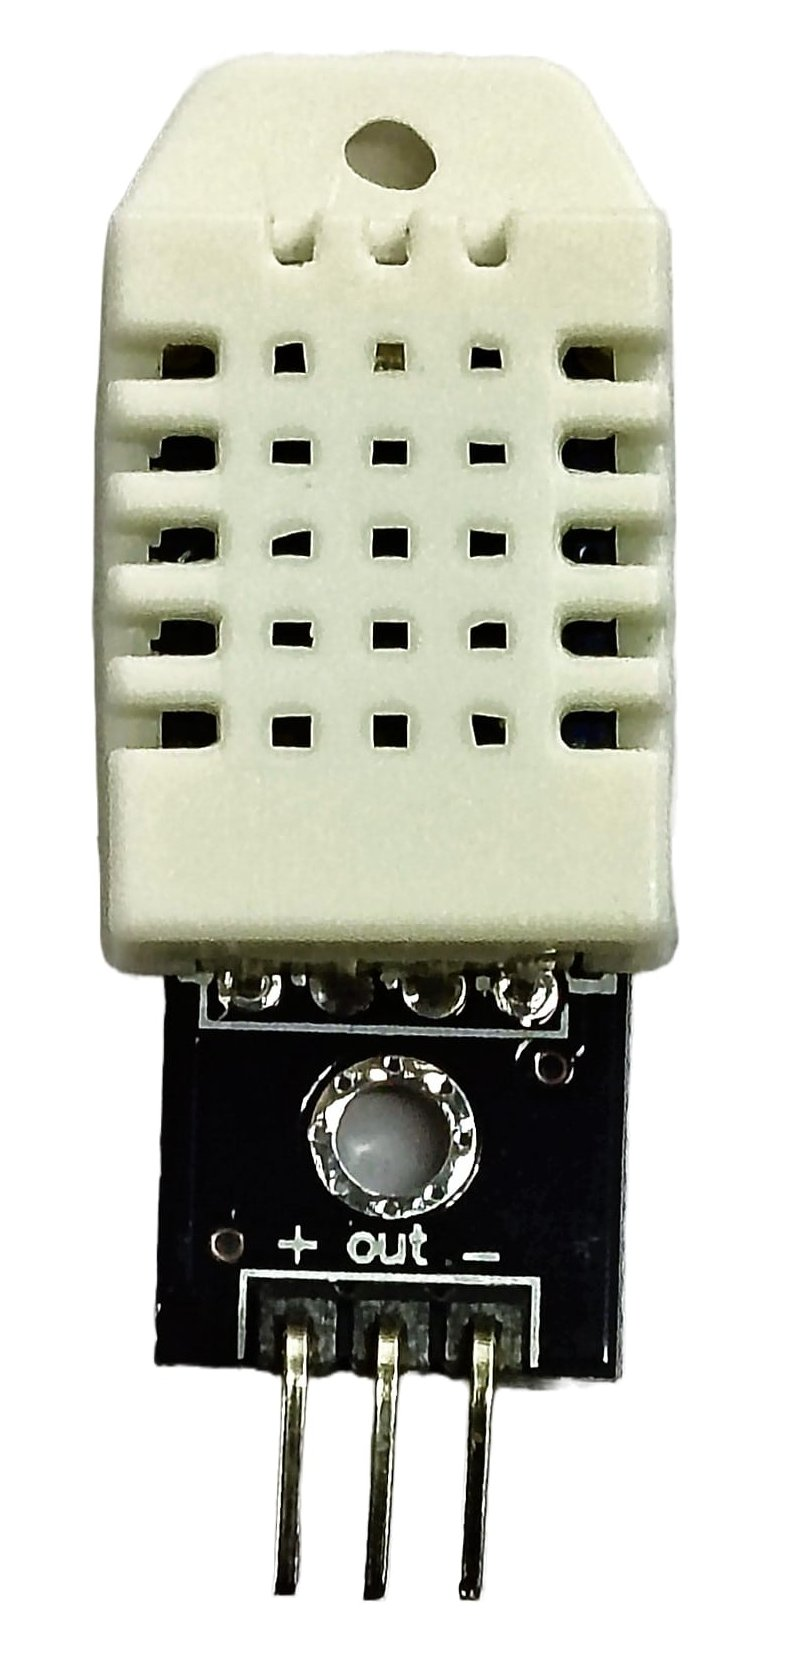
\includegraphics[width=.9\textwidth]{dht22}
        \end{column}
        \begin{column}{.6\textwidth}
            Mesure température (\(\pm\) 0.5°C) et d'humidité
            (\(\pm\) 2\%)

            \bigskip

            Brancher le DHT22 au GPIO:
            \begin{itemize}
                \item[\texttt{+}] \(\rightarrow\) 5V
                \item[\texttt{out}] \(\rightarrow\) GPIO 4 (pin 7)
                \item[\texttt{-}] \(\rightarrow\) GND
            \end{itemize}

            \bigskip
            Utilise un protocole 1-fil propriétaire

            \alert{\(\rightarrow\) nécessite une librairie dédiée}
        \end{column}
    \end{columns}
\end{frame}

\begin{frame}{Installer des librairies Python}{\texttt{pip} et \texttt{venv}}
    \cmd{pip} est le gestionnaire de paquets Python
    \begin{itemize}
        \item \cmd{pip}\args{ install librairie}: installer une librairie
        \item \cmd{pip}\args{ list}: lister les librairies installées
        \item \cmd{pip}\args{ uninstall librairie}: désinstaller une
              librairie
    \end{itemize}

    \bigskip
    \texttt{venv} est un module Python pré-installé pour créer des
    environnements virtuels
    \begin{itemize}
        \item isoler les dépendances d'un projet
        \item utiliser différentes versions de python ou de librairies
    \end{itemize}
\end{frame}

\begin{frame}[fragile]{Mise en place pour le DHT22}{Création d'un environnement
        virtuel et installation de librairies}
    Se déplacer dans un dossier de travail, puis:
    \bigskip

    \begin{enumerate}
        \item Créer un environnement virtuel nommé \texttt{pienv}

              \cmd{python}\args{ -m venv pienv -{}-system-site-packages}
        \item Vérifier que l'environnement virtuel a été crée

              \cmd{ls} \(\rightarrow\) chercher un dossier \texttt{pienv}
        \item Activer l'environnement virtuel

              \cmd{source}\args{ pienv/bin/activate}
        \item Installer la librairie

              \cmd{pip}\args{ install adafruit-circuitpython-dht}
    \end{enumerate}
\end{frame}

\begin{frame}[fragile]{Lire les mesures du DHT22}
    \begin{lstlisting}
import adafruit_dht
import board

# Creer un objet DHT22 sur le port GPIO4 (pin 7)
dht = adafruit_dht.DHT22(board.D4)

# Lire la temperature et l'humidite
print("Temperature:", dht.temperature, "C")
print("Humidite:", dht.humidity, "%")
    \end{lstlisting}

    Exercices:
    \begin{itemize}
        \item afficher les mesures toutes les secondes
        \item afficher les mesures lorsqu'on appuie sur le bouton
        \item allumer la LED si la température dépasse un seuil
    \end{itemize}
\end{frame}

\begin{frame}{Les HATs}{Bien plus que des chapeaux}
    Hardware Attached on Top (HAT): extensions matérielles pour Raspberry Pi
    \begin{itemize}
        \item se connectent sur les broches GPIO
        \item offrent des fonctionnalités variées
    \end{itemize}

    \bigskip
    \begin{columns}
        \begin{column}{.3\textwidth}
            \centering
            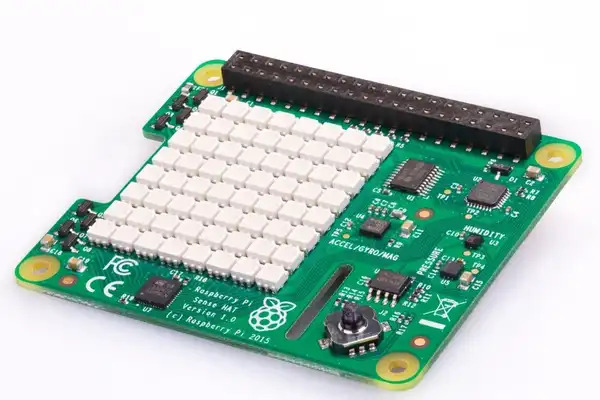
\includegraphics[width=\textwidth]{hat_sense}

            Sense HAT
        \end{column}
        \begin{column}{.3\textwidth}
            \centering
            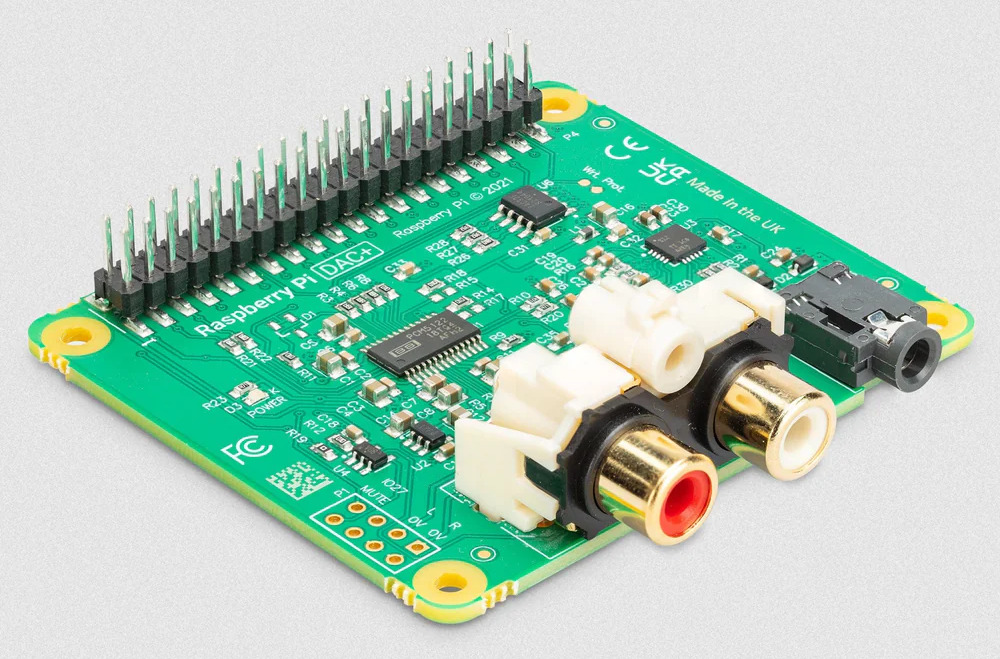
\includegraphics[width=\textwidth]{hat_dac}

            DAC+ HAT
        \end{column}
        \begin{column}{.3\textwidth}
            \centering
            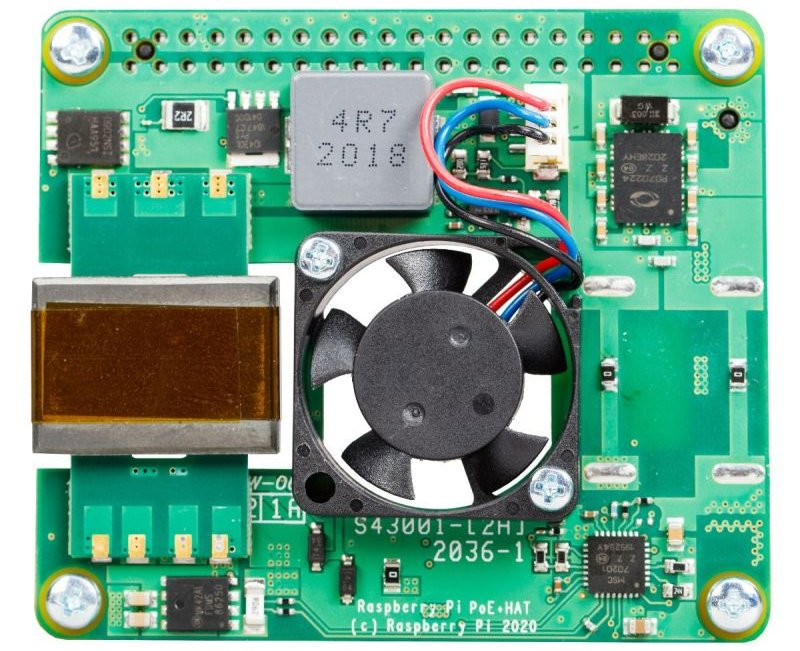
\includegraphics[width=\textwidth]{hat_poe}

            PoE+ HAT
        \end{column}
    \end{columns}
\end{frame}

\end{document}
